\chapter[Spectrum Database]{Spectrum Database}
%\addcontentsline{toc}{chapter}{Chapter 3\\Spectrum Database}
\label{chapter:Database}
In Chapter \ref{chapter:Database}, the overview of spectrum sharing with spectrum database and the measurement-based Spectrum Database proposed by our laboratory. And a problem of Spectrum Database Construction is described.

\section{Overview of Spectrum Sharing with Spectrum Database}
For further improving the performance for spectrum sharing, Federal Communications Commission(FCC), an independent agency of the United States government,proposed to fully utilize spectrum database for supporting spectrum sharing. Secondary User should obtain own postion by Global Position System(GPS) and access to database. FCC has already released the detailed rule of construction and managementfor TV broadcasting White Space and some service provider corporation have already established spectrum databases.\cite{ref:fcc,ref:google,ref:microsoft}. However, FCC-defined Database is determined by following a specified propagation model and only stores the decision information whether the White Space can be utilized or not at each position based on the calculation result from the propagation model. Based on the information from GPS, Secondary User accesses to the spectrum database to obtain the White Space information. Because interference towards Primary User is designed by managing geographic White Space conservatively, FCC-defined Spectrum Database is only treated as overlay spectrum sharing. Consequently, as the interference margin is set too large, the calculation of interfernce power with following a detailed propagation model is not considered, which is described in Chapter \ref{chapter:CR} that the spectrum usage efficiency improvement has a upper limit.
\begin{figure}[!htp]
\begin{center}
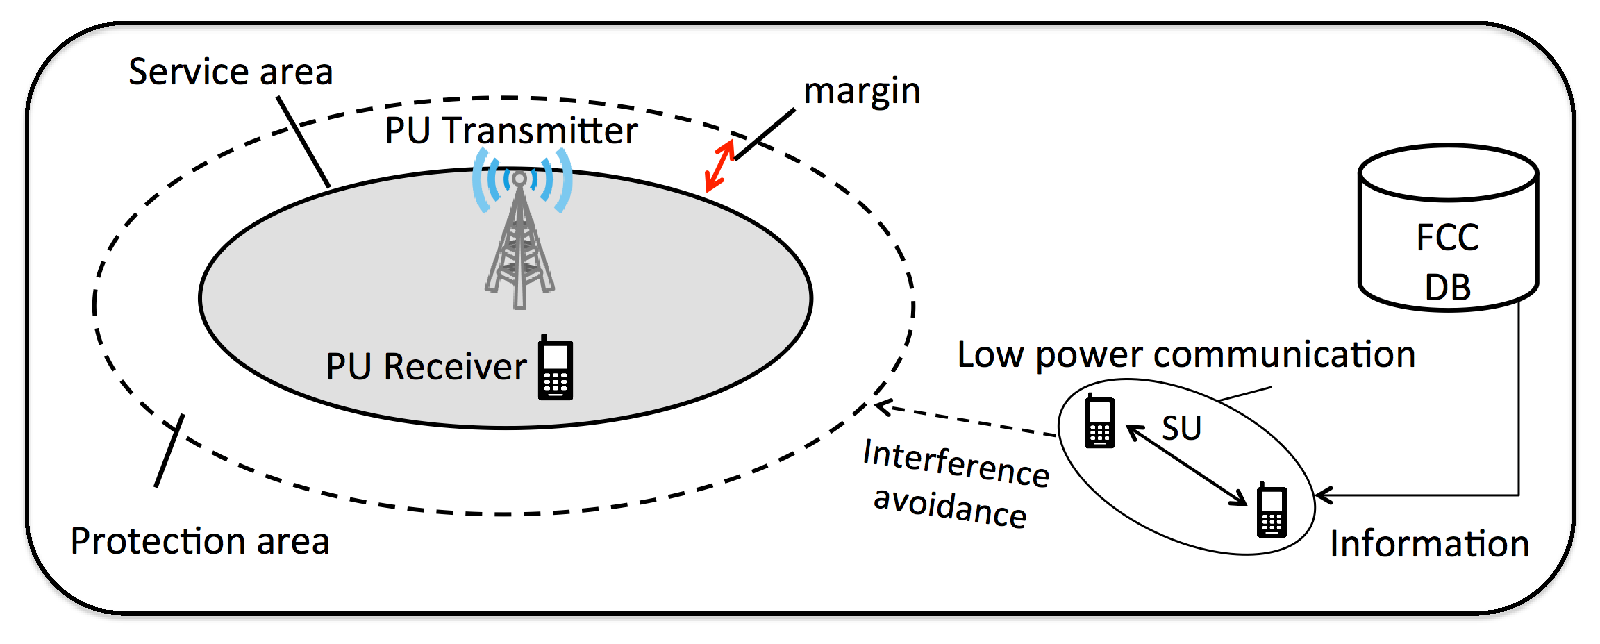
\includegraphics[width=120mm,clip]{fcc_sdb.eps}
\caption{FCC-defined Spectrum Database.}
\label{fig:fcc-defined_sdb}
\end{center}
\end{figure}

\section{Measurement-based Spectrum Database}
To obtain a large improvement on spectrum usage efficiency, underlay spectrum sharing spectrum database should be considered instead of overlay type. Thus, a more advanced radio environment database besides FCC-defined spectrum database is required for providing not only the White Space information, but also the information about Primary, such as Modulation and Coding Scheme(MCS) and transmision power, a more detailed propagation model, estimation error and the position of Primary receiver and so on.

\begin{figure}[!htp]
\begin{center}
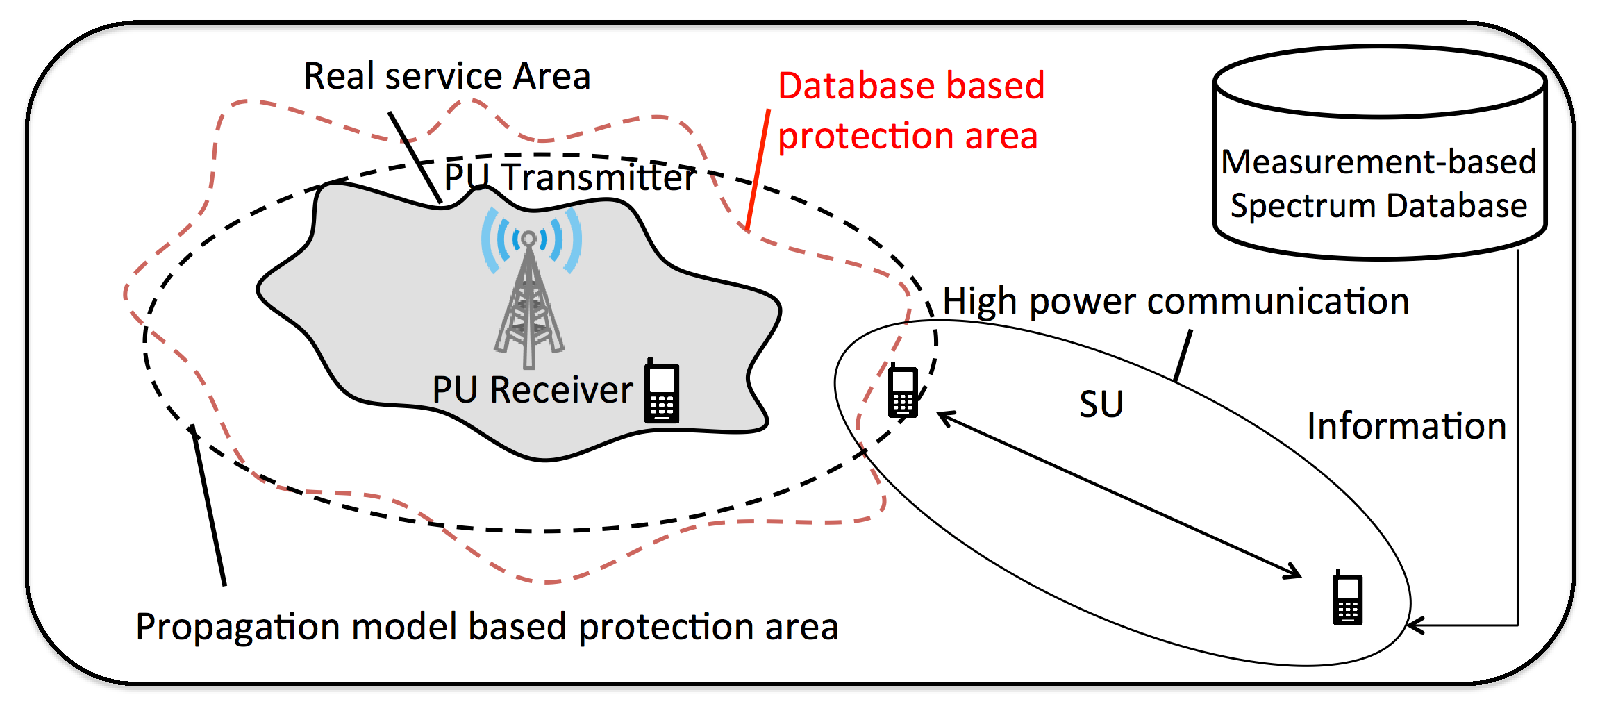
\includegraphics[width=120mm,clip]{asdb.eps}
\caption{Measurement-based Spectrum Database.}
\label{fig:asdb}
\end{center}
\end{figure}



    \subsection{Spectrum Datbase Construction based on Energy Detection}

\section{Problem of Spectrum Database Construction }

